\let\negmedspace\undefined
\let\negthickspace\undefined
\documentclass[journal,onecolumn]{IEEEtran}

\usepackage[a5paper, margin=10mm]{geometry} % Safe with onecolumn
\usepackage{lmodern} % Better fonts (optional but recommended)
\usepackage{tfrupee} % Rupee symbol package

% Header fix
\setlength{\headheight}{12pt} % Safe value
\setlength{\headsep}{0pt}     % Reduce gap

\usepackage{gvv-book}
\usepackage{gvv}
\usepackage{cite}
\usepackage{amsmath,amssymb,amsfonts,amsthm}
\usepackage{algorithmic}
\usepackage{graphicx}
\usepackage{textcomp}
\usepackage{xcolor}
\usepackage{txfonts}
\usepackage{listings}
\usepackage{enumitem}
\usepackage{mathtools}
\usepackage{gensymb}
\usepackage{comment}
\usepackage[breaklinks=true]{hyperref}
\usepackage{tkz-euclide} 
\usepackage{listings}
% \usepackage{gvv}                                        
\def\inputGnumericTable{}                                 
\usepackage[latin1]{inputenc}                                
\usepackage{color}                                            
\usepackage{array}                                            
\usepackage{longtable}                                       
\usepackage{calc}                                             
\usepackage{multirow}                                         
\usepackage{hhline}                                           
\usepackage{ifthen}                                           
\usepackage{lscape}

\usepackage{amsmath,amssymb}
\usepackage{booktabs}
\usepackage{tikz}
\usetikzlibrary{arrows.meta,angles,quotes}

\begin{document}

\bibliographystyle{IEEEtran}
\vspace{3cm}

\title{4.10.16}
\author{EE25BTECH11014 - Bhoomika Lokesh}
% \maketitle
% \newpage
% \bigskip
{\let\newpage\relax\maketitle}

\renewcommand{\thefigure}{\theenumi}
\renewcommand{\thetable}{\theenumi}
\setlength{\intextsep}{10pt} % Space between text and floats

% Remove this line so equations use default numbering (1, 2, 3,...)
% \numberwithin{equation}{enumi}
\numberwithin{figure}{enumi}
\renewcommand{\thetable}{\theenumi}


\textbf{Question:} Solve the given system of linear equations:
\begin{align}
     x-3y-7=0\\  3x-3y-15=0 
\end{align}
\textbf{Solution:}\\
The given equations of line can be expressed as:\\
\begin{center}
   $ \vec{n^T}\vec{x}=c$
\end{center}

\begin{align}
 \myvec{1&-3}\myvec{x\\y}=7\\
 \myvec{3 &-3}\myvec{x\\y}=15
\end{align}
The matrix we get by the above equations is as follows:
\begin{align}
     \myvec{1&-3\\3&-3}\myvec{x\\y}=\myvec{7\\15}
\end{align}
 The following is the augmented matrix which can be solved using Gaussian elimination.
 \begin{align}
       \myvec{\begin{array}{cc|c}
1 & -3 & 7 \\ 
3 & -3 & 15\end{array}} \xrightarrow{\;R_2\longrightarrow R_2-3R_1\;}       \myvec{\begin{array}{cc|c}
1 & -3 & 7 \\ 
0 & 6 & -6\end{array}}\\
\myvec{\begin{array}{cc|c}
1 & -3 & 7 \\ 
0 & 6 & -6\end{array}} \xrightarrow{\;R_2\longrightarrow \frac{R_2}{6}\;}
\myvec{\begin{array}{cc|c}
1 & -3 & 7 \\ 
0 & 1 & -1\end{array}}\\
\myvec{\begin{array}{cc|c}
1 & -3 & 7 \\ 
0 & 1 & -1\end{array}} \xrightarrow{\;R_1\longrightarrow R_1+3R_2\;} \myvec{\begin{array}{cc|c}
1 & 0 & 4 \\ 
0 & 1 & -1\end{array}} 
\end{align}

From the matrix,\\
\begin{align}
    \myvec{1&0\\0&1}\myvec{x\\y}=\myvec{4\\-1}\\
    \therefore \myvec{x\\y}=\myvec{4\\-1}
\end{align}
Hence the system of equations has a unique solution,$x=4$ and $y=-1$.


\begin{figure}[H]
\begin{center}
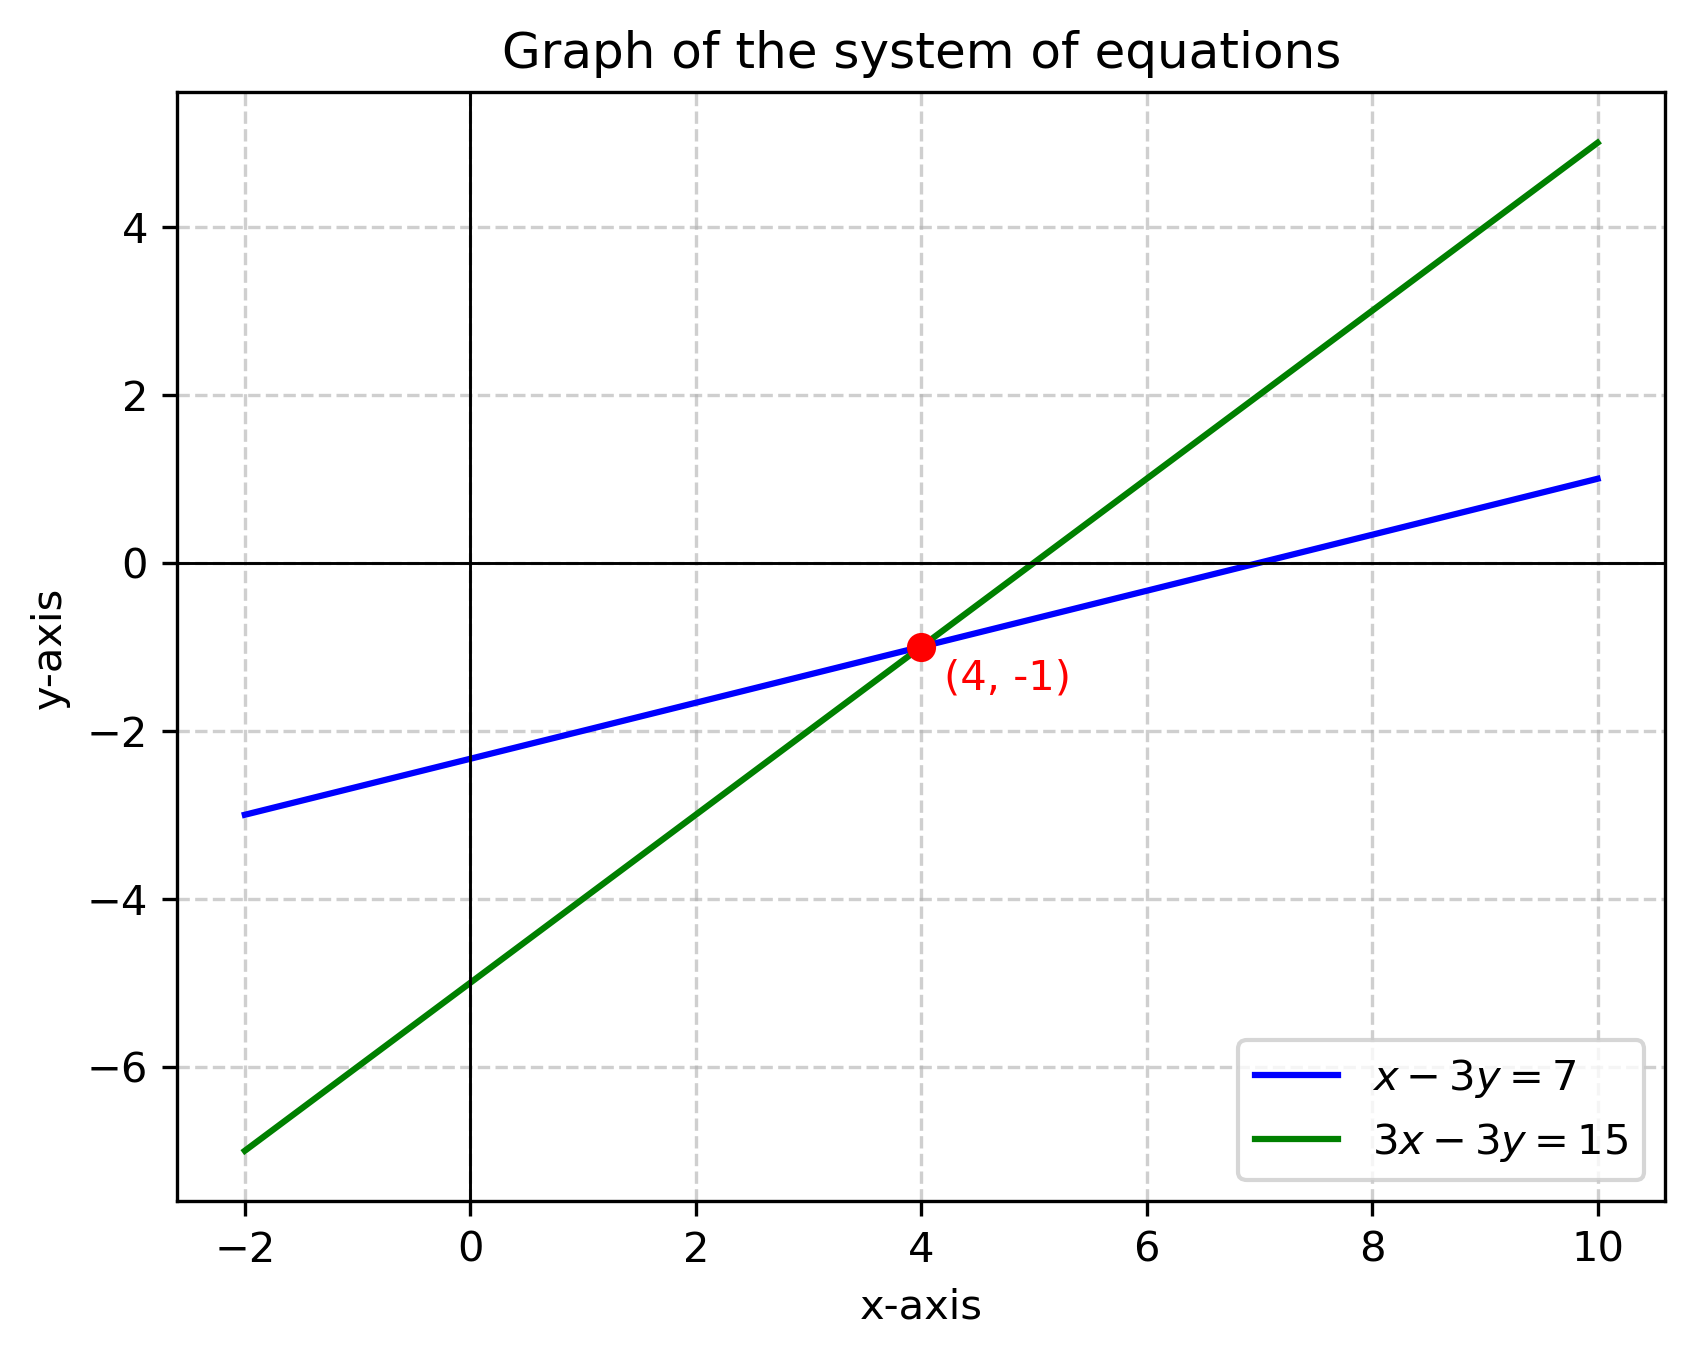
\includegraphics[width=0.7\columnwidth]{Figs/LE.png}
\end{center}
\caption{System of Linear Equations}
\label{fig:fig.py}
\end{figure}

\end{document}